\section{Masinõppe meetodite kvaliteedimõõtude võrdlus}
Uue meetodi kasutusele võtmine tähendab, et on olemas vanem juba kasutuses meetod. Võib osutuda otstarbekaks kasutada vanemat meetodit uue hindamisel. Vana meetodi asendamisel on eelkõige tähtis kas ja kui palju on uus meetod eelmisest parem. Väljaselgitamiseks võib uurida meetodite kvaliteedimõõtude vahesid.

Järgnevas laiendame eelmises peatükis sisse toodud tähistusi. Tähistagu $i$-ndat andmepunkti elementide paar $(x_i, y_i)$, kus $x_i$ tähistab andmepunkti tunnuseid ning $y_i$ andmepunkti klassi. Olgu $A$ uus ning $B$ varasem klassifitseerimismeetod, siis saame tähistada andmepunktile vastavad klassifikatsioone  $A(x_i)=a_i$ ja $B(x_i)=b_i$. Vaadeldes andmepunkti juhusliku suurusena $(X, Y)$ võib ka meetodite klassifikatsioone sellel vaadelda juhuslike suurustena $A$ ja $B$ ning meetodite kvaliteedimõõdud on defineeritud keskväärtuste kaudu läbi valemite \eqref{eq:õigsus}, \eqref{eq:täpsus} ja \eqref{eq:saagis}. Näiteks meetodi $B$ õigsus on $\accuracy_B=\mean{B=Y}$. Siit lähtuvalt saab meetodite erinevuse uurimisel vaadata meetodite kvaliteedimõõtude vahesid
\begin{align}
    \Delta\accuracy&=\mean{A=Y}-\mean{B=Y} \enspace, \label{eq:õigsus vahe} \\
    \Delta\precision&=\mean{A=Y|A=1}-\mean{B=Y|B=1} \enspace, \label{eq:täpsus vahe} \\
    \Delta\recall&=\mean{A=Y|Y=1}-\mean{B=Y|Y=1} \enspace. \label{eq:saagis vahe}
\end{align}

\subsection{Kvaliteedimõõtude vahede lähendid}
Kuna defineeritud vahede täpseid väärtusi on praktikas keeruline leida hinnatakse neid kasutades valimi keskmisi. Sealjuures on loomulik mõlema meetodi hindamiseks kasutada sama valimit. Ühelt poolt on see standardpraktika - tüüpiliselt hinnatakse masinõppemeetodite edukust fikseeritud testvalimite (\emph{benchmark}) peal. Teisalt tooks kahe valimi kasutamine vajaduse käsitsi märgendada rohkem andmepunkte ning lisab ka lõpptulemusse rohkem juhuslikkust. Kui vastav testvalim sisaldab $N$ andmepunkti, siis saab õigsuste vahe lähendi avaldada järgnevalt
\begin{align}
    \Delta\widehat{\accuracy}&=\frac{1}{N}\cdot\sum_{i=1}^{N}[a_i=y_i]-\frac{1}{N}\cdot\sum_{i=1}^{N}[b_i=y_i] \nonumber\\
    &=\frac{1}{N}\cdot\sum_{i=1}^{N}[a_i=y_i]-[b_i=y_i]\nonumber\\
    &=\frac{1}{N}\cdot\sum_{a_i\neq b_i}[a_i=y_i]-[b_i=y_i] \enspace. \label{eq:õigsus vahe lähend}
\end{align}
Saadud võrduses \eqref{eq:õigsus vahe lähend} on summa märgi all nullist erinev arv parajasti siis, kui meetodite klassifikatsioonid on erinevad. Sellest järeldub, et meetodite õigsuste vahe hindamiseks peab märgendama vaid andmepunkte, kus $a_i\neq b_i$. Näiteks kui meetodid on üle $90\%$ õigsustega võivad nende klassifikatsioonid erineda maksimaalselt $20\%$ andmetest. Sellisel juhul peab märgendama vaid iga viienda andmepunkti. Veelgi enam, kuna iga summa liige valemis  \eqref{eq:õigsus vahe lähend} on $\pm 1$, saab hinnata $\Delta\widehat{\accuracy}$ ilma ühtegi andmepunkti märgendamata
\begin{equation}
    \label{eq:õigsus vahe lähend tõke}
    |\Delta\widehat{\accuracy}|\leq\frac{\#\{i: a_i\neq b_i\}}{N} \enspace,
\end{equation}
kus murru lugejas tähistab $\#$ hulga suurust. Seega on võimalik veenduda, kas kaks algoritmi üldse õigsuse poolest erinevad andmepunktide tegelikke klasse teadmata.

Analoogselt õigsusele võib avaldada ka valimipõhiste täpsushinnangute vahe
\begin{equation}
    \label{eq:täpsus vahe lähend kole}
    \Delta\widehat{\precision}=\frac{\sum\limits_{i=1}^{N}[a_i=1]\cdot[y_i=1]}{\sum\limits_{i=1}^N[a_i=1]}-
    \frac{\sum\limits_{i=1}^{N}[b_i=1]\cdot[y_i=1]}{\sum\limits_{i=1}^N [b_i=1]} \enspace,
\end{equation}
mille edasise lihtsustamise muudab raskeks erinevus murru nimetajates. Kuna tehniliselt ei pea täpsuse hindamisel kasutama sama testvalimit mõlema algoritmi jaoks, siis võib esialgset testvalmit kitsendada nii, et murru lugejad langevad kokku
\begin{equation*}
    \sum\limits_{i=1}^{N_A}[a_i=1]=S=\sum\limits_{i=1}^{N_B}[b_i=1] \enspace,
\end{equation*}
ning $N=\max(N_A, N_B)$.
Selline lähenemine on samaväärne valikumeetodi põhjal kahe $S$ andmepunktise valimi moodustamisega, kus vastuvõtutingimused on vastavalt $a_i=1$ ja $b_i=1$. Seda arvestades saab valemi \eqref{eq:täpsus vahe lähend kole} viia lihtsustatud kujule
\begin{equation}
     \Delta\widehat{\precision}=\frac{1}{S}\cdot\sum\limits_{i=1}^{N_A}[a_i=1]\cdot[y_i=1]-\frac{1}{S}\cdot\sum\limits_{i=1}^{N_B}[b_i=1]\cdot[y_i=1] \enspace,
\end{equation}
kus $a_i$ on määratud vaid esimesel $N_A$ ja $b_i$ on määratud vaid esimesel $N_B$ andmepunktil. Seega on $a_i$ ja $b_i$ väärtus kõigi $N$ punkti seas kas määramata, $0$ või $1$. Siit lähtuvalt
\begin{align}
    \Delta\widehat{\precision}&=\frac{1}{S}\cdot\left(\sum_{\substack{a_i=1\\ b_i=1}}[y_i=1]+\sum_{\substack{a_i=1\\ b_i\neq 1}}[y_i=1]-\sum_{\substack{a_i=1\\ b_i=1}}[y_i=1]-\sum_{\substack{a_i\neq 1\\ b_i=1}}[y_i=1]\right) \nonumber\\
    &=\frac{1}{S}\cdot\left(\sum_{\substack{a_i=1\\ b_i\neq 1}}[y_i=1]-\sum_{\substack{a_i\neq 1\\ b_i=1}}[y_i=1]\right) \nonumber\\
    &=\frac{1}{S}\cdot\sum_{a_i\neq b_i}[a_i=1]\cdot[y_i=1]-[b_i=1]\cdot[y_i=1] \enspace. \label{eq:täpsus vahe lähend}
\end{align}
Andmepunktide märgendamise mõttes on täpsuse vahe lähend \eqref{eq:täpsus vahe lähend} samaväärne õigsuse valemiga \eqref{eq:õigsus vahe lähend}, sest hinnangu arvutamiseks peab märgendama vaid andmepunkte, mille puhul $a_i\neq b_i$.

Täpsuse vahehinnangu praktiline arvutamine algab $S$ fikseerimisest. Seejärel tuleb valimile rakendada meetodeid kuni kumbki on $S$ andmepunkti positiivseks klassifitseerinud. Märgendama peab valimi andmepunktid, mille puhul on olemas mõlema meetodi klassifikatsioonid, mis on üksteisest erinevad. Nüüd on võimalik arvuta summa liikmete väärtused ning seejärel hinnang täpsuste vahele. Sellega on oluliselt vähendatud märgendamist vajavate andmete hulka.

Saagise vahe avaldub sarnaselt täpsusele, lähtudes valemist
\begin{equation*}
    \Delta\widehat{\recall}=\frac{\sum\limits_{i=1}^{N}[a_i=1]\cdot[y_i=1]}{\sum\limits_{i=1}^{N}[y_i=1]}-\frac{\sum\limits_{i=1}^{N}[b_i=1]\cdot[y_i=1]}{\sum\limits_{i=1}^{N}[y_i=1]} \enspace,
\end{equation*}
kus erinevalt täpsusest on murdude nimetajad definitsiooni järgi võrdsed. Tähistagu nimetajas olevat summat
\begin{equation*}
    T=\sum_{i=1}^N[y_i=1] \enspace.
\end{equation*}
Korrates täpsuse valemi \eqref{eq:täpsus vahe lähend} tuletamisega analoogset mõttekäiku, võib esitada saagise vahe hinnangu kujul
\begin{equation}
    \label{eq:saagis vahe lähend}
     \Delta\widehat{\recall}=\frac{1}{T}\cdot\sum_{a_i\neq b_i}[a_i=1]\cdot[y_i=1]-[b_i=1]\cdot[y_i=1] \enspace. 
\end{equation}
Märgendamise seisukohalt on $T$ arvutamine kulukas, kuna iga summa liikme puhul peab teadma andmepunkti tegelikku klassi. Kõigi $N$ andmepunkti manuaalne märgendamine on väga ressursimahukas. 
Alternatiiviks on väiksema valimi põhjal positiivse klassi esinemise sageduse ennustamine. See on võimalik vaid siis kui positiivse klassi esinemise sagedus on piisavalt suur. Kui positiivse klassi esindajad on sagedusega $1:1000$, siis on tarvis adekvaatse hinnangu saamiseks läbi vaadata üle kümnetuhande andmepunkti. Seega on valemi \eqref{eq:saagis vahe lähend} praktiline rakendamine raskendatud veelgi madalama esinemissagedusega sündmuste korral.

\subsection{Õigsuste vahe lähendamine}
Siiani on lähendid kvaliteedimõõtude vahele avaldatud vahetult läbi vahe oodatud väärtuse definitsiooni. Tehes teisendusi vahe definitsioonis antud avaldises on võimalik see eraldada mitmeks komponendiks. Vahe lähendi saamiseks on ka võimalik lähendada iga komponenti eraldi ning nende põhjal arvutada hinnang vahele.

Olgu olemas kaks klassifitseerimismeetodit koos juhusliku andmepunkti $Y$ klassifitseerimisele vastavate juhuslike suurustega $A$ ja $B$. Siis saab valemi \eqref{eq:õigsus vahe} kirjutada lahti vastavalt definitsioonile
\begin{equation}
    \label{eq:õigus vahe definitsiooni järgi keskväärtuste kaudu}
    \Delta\accuracy=\mean{A=Y}-\mean{B=Y}=\mean{[A=Y]-[B=Y]} \enspace.
\end{equation}
Tähistagu $Z$ valemis \eqref{eq:õigus vahe definitsiooni järgi keskväärtuste kaudu} viimase keskväärtusmärgi all olevat juhuslikkus suurust, ehk $Z=[A=Y]-[B=Y]$. Analoogselt võib valemis \eqref{eq:õigsus vahe lähend} oleva summa liikmeid tõlgendada juhuslike suurustena $Z_i=[a_i=y_i]-[b_i=y_i]$. Arvestades, et $Z_i$ on sõltumatud ning sama jaotusega kui $Z$, on lihtne näha, et lähendi \eqref{eq:õigsus vahe lähend} keskväärtus on
\begin{equation}
    \mean{\Delta\widehat{\accuracy}}=\frac{1}{N}\cdot\sum_{i=1}^N\cdot\mean{Z_i}=\Delta\accuracy \enspace.
\end{equation}
See tähendab, et $\widehat{\accuracy}$ on nihketa hinnang õigsuste vahele. Kuna meetodite erinevus avaldub sündmustes, kus meetodite klassifikatsioonid erinevad ($Z\neq 0$), võib $\Delta\accuracy$ avaldada selliste sündmuste kaudu
\begin{align*}
    \Delta\accuracy&=\prob{Z=0}\cdot\mean{Z \mid Z = 0}+\prob{Z \neq 0}\cdot\mean{Z \mid Z \neq 0} \\
    &=\prob{Z \neq 0}\cdot\mean{Z \mid Z \neq 0} \enspace.
\end{align*}
Edasiste arvutuste selgemaks esitamiseks on otstarbekas kasutusele võtta tähistused
\begin{align}
    \beta&=\prob{Z\neq0} \enspace, \label{eq:beta} \\
    \gamma&=\mean{Z \mid Z \neq 0} \enspace, \label{eq:gamma} \\
    \kappa&=\prob{Z=1|Z\neq0} \enspace. \label{eq:kappa}
\end{align}
Need kolm suurust pole sõltumatud parameetrid. Keskväärtuse definitsioonist lähtuvalt on $\gamma$ ja $\kappa$ omavahel seotud
\begin{equation*}
    \gamma=\mean{Z\mid Z \neq 0}=1\cdot\kappa-1\cdot(1-\kappa)=2\kappa-1 \enspace,
\end{equation*}
ning me saame esitada õigsuste vahe antud suuruste kaudu
\begin{equation}
    \label{eq:õigsus vahe tähistega}
    \Delta\accuracy=\beta\cdot\gamma=\beta\cdot(2\kappa-1) \enspace.
\end{equation}

Võrdusest (\ref{eq:õigsus vahe tähistega}) lähtuvalt on võimalik hinnata meetodite õigsuste vahet lähendades suurusi $\beta$ ja $\gamma$. Kuna $\beta = \prob{Z \neq 0}$ on tõenäosus saab seda hinnata statistilise tõenäosusena üle $N$ elemendilise valimi 
\begin{equation}
    \label{eq:beta lähend}
    \hat{\beta}=\frac{1}{N}\cdot\sum_{i=1}^{N}[Z_i\neq0]=\frac{1}{N}\cdot\sum_{i=1}^{N}[a_i\neq b_i] \enspace,
\end{equation}
\cite{rakendusstatisika-algkursus}.
Lähendi leidmisel summa märgi alune juhuslik suurus võtab väärtusi $0$ ja $1$. See tähendab, et lähendi absoluutse ja relatiivse vea hinnangud on leitavad eelmises peatükis kirjeldatud meetodeid kasutades.

Lähend tinglikule keskväärtusele $\gamma=\mean{Z\mid Z\neq 0}$ on leitav sarnaselt, valimikeskimisena, kus iga valimi andmepunkti korral $a_i \neq b_i$.
Olgu $K$ sellise valimi suurus, siis saab lähendi esitada kujul
\begin{equation}
    \label{eq:gamma lähend}
    \hat{\gamma}=\frac{1}{K}\cdot\sum_{i=1}^K [a_i=y_i]-[b_i=y_i] \enspace.
\end{equation}
Kuna lähendis $\hat{\gamma}$ on summa liikmete võimalikud väärtused $-1$ ja $1$, ei ole summa liikmed Bernoulli jaotusega. See-eest on ikka tegu binaarse tunnusega, mille põhjal saab defineerida uue Bernoulli jaotusega juhusliku suuruse, mis võtab väärtuse $0$ kui summeritav suurus võtab $-1$ ning muidu $1$
\begin{equation*}
    W = \frac{Z + 1}{2} \enspace,
\end{equation*}
mille puhul
\begin{align*}
    \prob{W=1}&=\prob{Z=1 \mid Z\neq 0}=\kappa \enspace, \\
    \prob{W=0}&=\prob{Z=-1 \mid Z\neq 0}=1-\kappa \enspace.
\end{align*}
Sündmusena on uus defineeritud suurus samaväärne vanaga, endiselt saab rakendada binoomjaotusel põhinevaid tulemusi eelmisest peatükist. Lähtudes võrrandist
\begin{equation*}
    \prob{\left| \frac{\hat{\gamma}}{\gamma} - 1 \right| \geq \varepsilon} = \alpha \enspace,
\end{equation*}
korrates sama mõttekäiku, mis valemi \eqref{eq:binoomjaotus relatiivne viga} puhul.

Leitud lähendite korrutis annab omakorda lähendi meetodite õigsuste vahele
\begin{equation*}
    \Delta\widehat{\accuracy}=\hat{\beta}\cdot\hat{\gamma} \enspace.
\end{equation*}
Vahe lähendi relatiivse vea dispersioon avaldub relatiivse vea korrutise omaduse \eqref{eq:korrutise relatiivne viga dispersioon ligikaudne} põhjal kujul
\begin{equation}
    \variance{\frac{\hat{\beta}\cdot\hat{\gamma}}{\beta\cdot\gamma}}\approx\variance{\frac{\hat{\beta}}{\beta}}+\variance{\frac{\hat{\gamma}}{\gamma}} \enspace,
\end{equation}
kus hinnangute $\hat{\beta}$ ja $\hat{\gamma}$ relatiivsete vigade dispersioonid on
\begin{align}
    \variance{\frac{\hat{\beta}}{\beta}}&=\frac{1}{N}\cdot\frac{1-\beta}{\beta} \enspace, \label{eq:beta relatiivne viga dispersioon} \\
    \variance{\frac{\hat{\gamma}}{\gamma}}&=\frac{1}{K}\cdot(\mean{Z^2 \mid Z\neq 0}-\mean{Z \mid Z\neq 0}^2)=\frac{1}{K}\cdot(1-\gamma^2) \enspace. \label{eq:gamma relatiivne viga dispersioon}
\end{align}

\begin{figure}[H]
    \begin{center}
        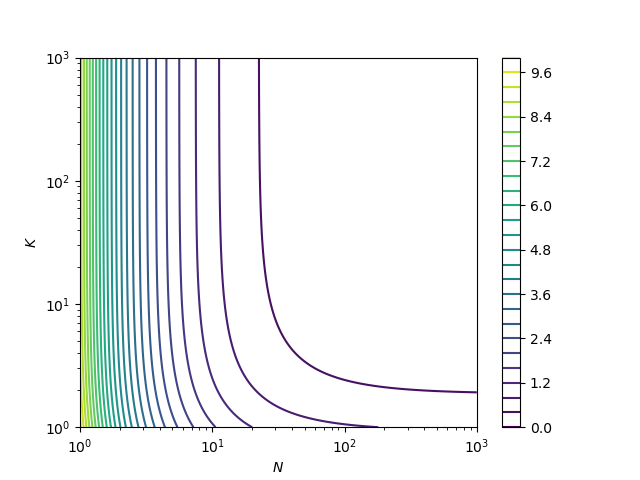
\includegraphics[width=\textwidth]{oigsus_vahe_relatiive_viga_dispersioon.png}  
    \end{center}
    \caption{Õigsuste vahe lähendi relatiivse vea dispersioon juhusliku valimi suuruse $N$ ning märgendatud tingliku $(a_i \neq b_i)$ valimi suuruse $K$ suhtes. Juhul kui $\Delta\accuracy=5\%$ ja $\beta=10\%$. Heledus tähistab dispersiooni.}
    \label{fig:õigsus vahe lähend relatiivne viga dispersioon}
\end{figure}

Jooniselt \ref{fig:õigsus vahe lähend relatiivne viga dispersioon} ning vahetulemuste \eqref{eq:beta relatiivne viga dispersioon} ja \eqref{eq:gamma relatiivne viga dispersioon} kaudu on näha, et $\Delta\widehat{\accuracy}$ relatiivse vea dispersioon kahaneb valimisuuruste kasvades. Telgedel olevatest suurustest tähistab $N$ valimi suurust, mida ei pea märgendama. Kuna sellise valimi leidmine ei ole keeruline võib eeldada, et $N$ on fikseeritud ja küllaltki suur. Oluline on aga suurus $K$, mis tähistab märgendamist vajavate andmepunktide arvu. Märgendatud valimi suuruse prognoosimiseks fikseeritud $N$ põhjal võib uurida olukorda, kus saavutatakse võrdsed lähendite $\hat{\beta}$ ja $\hat{\gamma}$ dispersioonid
\begin{equation}
    \label{eq:võrdsed vahe relatiivse vea dispersioonid}
    \frac{1}{N}\cdot\frac{1-\beta}{\beta}=\frac{1}{K}\cdot(1-\gamma^2) \enspace.
\end{equation}
Kuna $\Delta\accuracy=\beta\cdot\gamma$, on valem \eqref{eq:võrdsed vahe relatiivse vea dispersioonid} esitatav kujul
\begin{equation}    
    K = N \cdot \frac{\beta}{1-\beta} \cdot \left( 1 - \frac{(\Delta\accuracy)^2}{\beta^2} \right) \enspace,
\end{equation}
mille põhjal on võimalik hinnata märgendatud valimi suurust.

\subsection{Saagiste vahe lähendamine}
Saagise puhul on hinnangu \eqref{eq:saagis vahe lähend} analüüsimine keerulisem, kuna saagise definitsioonis on tinglik keskväärtus. Valemile \eqref{eq:õigsus vahe tähistega} analoogi tuletamiseks peab kõigepealt eraldama saagise definitsioonist tingliku jaotuse
\begin{align*}
    \mean{A=Y \mid Y=1}&=\mean{A=1 \mid Y=1}=\prob{A=1 \mid Y=1}\enspace, \\
    \mean{B=Y \mid Y=1}&=\mean{B=1 \mid Y=1}=\prob{B=1 \mid Y=1}\enspace,
\end{align*}
millest saab tuletada
\begin{align*}
    \mean{A=Y \mid Y=1}&=\frac{\prob{A=1 \land Y=1}}{\prob{Y=1}} =\frac{\mean{[A=1]\cdot[Y=1]}}{\mean{Y=1}} \enspace.
\end{align*}
Analoogselt meetodi $B$ puhul
\begin{align*}
    \mean{A=Y \mid Y=1}&=\frac{\prob{B=1 \land Y=1}}{\prob{Y=1}} =\frac{\mean{[B=1]\cdot[Y=1]}}{\mean{Y=1}} \enspace.
\end{align*}
Nende kahe võrduse põhjal võib saagiste vahe esitada kujul
\begin{align*}
    \Delta\recall&=\mean{A=Y \mid Y=1}-\mean{B=Y \mid Y=1} \\
    &=\frac{\mean{[A=1]\cdot[Y=1]-[B=1]\cdot[Y=1]}}{\mean{Y=1}} \enspace.
\end{align*}
Sellest saab järeldada algse saagise lähendi valemi \eqref{eq:saagis lähend} põhjal, et ka saagiste vahe lähend \eqref{eq:saagis vahe lähend} on nihketa. Kuid sellisel kujul esitatud vahele $\Delta\recall$ ei ole lähendi leidmine märgendamise seisukohalt veel kõige parem.

Kehtivad seosed
\begin{align*}
    \mean{[A=1][Y=1]} &= \mean{[A=1][Y=1][B=1]} + \mean{[A=1][Y=1][B=0]} \enspace, \\
    \mean{[B=1][Y=1]} &= \mean{[B=1][Y=1][A=1]} + \mean{[B=1][Y=1][A=0]} \enspace,
\end{align*}
nende seoste ja keskväärtuse definitsiooni põhjal on saagise vahe lugeja esitatav korrutisena tõenäosusest ja tinglikust keskväärtusest
\begin{align*}
    &\mean{[A=1][Y=1]-[B=1][Y=1]} \\
    &=\mean{[A=1][Y=1][A\neq B]-[B=1][Y=1][A\neq B]} \\
    &=\prob{A\neq B}\cdot\mean{[A=1][Y=1]-[B=1][Y=1] \mid [A\neq B]} \enspace.
\end{align*}
Edasiste arvutuste selgemaks esitamiseks on jällegi hea kasutusele võtta tähistused
\begin{align*}
    \beta&=\prob{A\neq B} \enspace, \\
    \nu&=\prob{Y=1} \enspace, \\
    \eta&=\mean{[A=1][Y=1]-[B=1][Y=1] \mid [A\neq B]} \enspace,
\end{align*}
mille kaudu saab esitada saagiste vahe
\begin{equation}
    \label{eq:saagis vahe tähistega}
    \Delta\recall=\frac{\beta\cdot\eta}{\nu} \enspace.
\end{equation}

Tulemuse \eqref{eq:saagis vahe tähistega} põhjal on võimalik meetodite saagiste vahet hinnata lähendades suurusi $\beta$, $\nu$ ja $\eta$. Tõenäosuse $\beta$ puhul on hinnang leitav samamoodi nagu \eqref{eq:beta lähend} eelmises alampeatükis. Ning $\nu$ lähend sarnaselt üle $N$ suuruse juhusliku valimi
\begin{align*}
    \hat{\beta}&=\sum_{i=1}^N [a_i \neq b_i] \enspace, \\
    \hat{\nu}&=\sum_{i=1}^N [y_i = 1] \enspace.
\end{align*}
Tinglikku keskväärtust $\eta$ on võimalik lähendada valimikeskmisena üle tingliku valimi, kus $a_i \neq b_i$. Olgu selle valimi suurus $K$, siis
\begin{equation*}
    \hat{\eta}=\frac{1}{K}\cdot\sum_{i=1}^K [a_i=1][y_i=1]-[b_i=1][y_i=1] \enspace.
\end{equation*}
Kuna hinnangute $\hat{\beta}$ ja $\hat{\nu}$ puhul on summa liikmete võimalikud väärtused $0$ ja $1$, on lähendite absoluutse ja relatiivse vea hinnangud leitavad meetoditega eelmisest peatükist. Kuna lähendi $\hat{\eta}$ puhul on summa liikmete võimalikud väärtused $-1$, $0$, ja $1$, ei saa rakendada binoomjaotusel põhinevaid tulemusi. See-eest on endiselt võimalik kasutada Höffdinig võrratust lähendi absoluutse vea jaoks, seekord tõketega $-1$ ja $1$, mille põhjal avaldub valimi vajalik suurus
\begin{equation*}
    K \geq - \frac{2}{\varepsilon^2} \cdot \ln{\left( \frac{\alpha}{2} \right)} \enspace,
\end{equation*}
kus $\varepsilon$ tähistab absoluutse vea absoluutväärtuse maksimaalset lubatud suurust ning $\alpha$ olulisust.

Relatiivse vea korrutise \eqref{eq:korrutise relatiivne viga dispersioon ligikaudne} ja jagatise \eqref{eq:jagatis relatiivne viga dispersioon} dispersiooni omaduste põhjal võib saagise vahe hinnangu relatiivse vea dispersiooni esitada summana
\begin{equation*}
    \variance{\frac{\hat{\beta}\cdot\hat{\eta}}{\hat{\nu}}:\frac{\beta\cdot\eta}{\nu}}\approx\variance{\frac{\hat{\beta}}{\beta}}+\variance{\frac{\hat{\nu}}{\nu}}+\variance{\frac{\hat{\eta}}{\eta}} \enspace,
\end{equation*}
millest
\begin{equation*}
    \variance{\frac{\hat{\beta}}{\beta}}=\frac{1}{N}\cdot\frac{1-\beta}{\beta},\qquad \variance{\frac{\hat{\nu}}{\nu}}=\frac{1}{N}\cdot\frac{1-\nu}{\nu} \enspace. \\
\end{equation*}
Ning kuna $\eta$ relatiivse vea dispersioon siin kasutusel olevate tähiste kaudu ilusalt ei esitu, võib seda lähendada ka kasutades valimidispersiooni valemit.

\subsection{Täpsuste vahe lähendamine}
Täpsuse jaoks on võrrandi \eqref{eq:saagis vahe tähistega} analoogi tuletamine keeruline, sest täpsuste vahe lähendis on summa liikmed mittesõltumatud. Üheks võimalikuks lahenduseks täpsuse hindamisel on kahesammuline lähenemine, kus hinnatakse esmalt lähendi \eqref{eq:täpsus vahe lähend kole} dispersiooni funktsioonina valikumeetodi abil saadud $S$ elemendilisest valimist (kahe keskmise vahe) ning seejärel lähendatakse selle optimeeritud esitust \eqref{eq:täpsus vahe lähend} veelgi väiksema $K$-elemendilise juhuvalimiga. Kuna saadud lahendus ei ole elegantne ning kõik sammud iseseisvalt on analoogsed peatükis \ref{section:kvaliteedimõõtude veahinnangud} saadud tulemustega, siis ei ole seda antud töös pikemalt käsitletud.